\documentclass[10pt,a4paper]{article}

\newcommand{\buildmode}{simple}
\InputIfFileExists{version.tex}{}{}
\providecommand{\version}{eleve}

\usepackage{feuilleinterro}
\usepackage{tikz}
\usepackage{tkz-tab}

\renewcommand{\niveau}{SBM 2}
\renewcommand{\chapitre}{Dérivation}
\renewcommand{\numchap}{0.3}
\renewcommand{\theme}{Dérivation}

\newcommand{\tangentegraph}[6]{%
  % #1 domaine courbe min, #2 domaine courbe max, #3 expression f(x) en \x
  % #4 domaine tangente min, #5 domaine tangente max, #6 expression tangente en \x
  \begin{tikzpicture}[scale=0.62]
  \draw[step=1cm,gray!30,very thin] (-2,-4) grid (5,6);
  \draw[->] (-2,0) -- (5.4,0) node[right] {\(x\)};
  \draw[->] (0,-4) -- (0,6.4) node[above] {\(y\)};
  \foreach \x in {-2,-1,1,2,3,4,5} \draw (\x,-0.08) -- (\x,0.08) node[below=2pt] {\scriptsize \x};
  \foreach \y in {-4,-3,-2,-1,1,2,3,4,5,6} \draw (-0.08,\y) -- (0.08,\y) node[left=2pt] {\scriptsize \y};
  \node[below left] at (0,0) {\scriptsize O};
  \draw[domain=#1:#2,smooth,variable=\x,blue,thick] plot ({\x},{#3}) node[above right] {\(\mathcal{C}_f\)};
  \draw[domain=#4:#5,variable=\x,red,thick] plot ({\x},{#6});
  }

\begin{document}

\interroversion{A}

\textbf{Exercice 1 -- Nombre dérivé lu graphiquement \hfill /1}

La courbe \(\mathcal{C}_f\) d'une fonction \(f\) et sa tangente \(T\) au point \(A\) d'abscisse \(2\) sont tracées ci-dessous.

\`A l'aide du graphique, déterminer \(f'(2)\).

\begin{center}
\tangentegraph{-1}{3}{\x*\x-2*\x+3}{0.5}{3.5}{2*\x-1}
\fill (2,3) circle (2pt);
\node[below right] at (2.05,2.95) {\(A\)};
\node[red] at (0.5,1) {\(T\)};
\end{tikzpicture}
\end{center}

Réponse~: \(f'(2)=\) \dotfill

\textbf{Exercice 2 -- Signe de la dérivée et variations \hfill /1}

On donne ci-dessous le tableau de variations d'une fonction \(f\) définie sur \([-3;4]\). En déduire, en le complétant, le tableau de signes de \(f'\) sur ce même intervalle.

\begin{center}
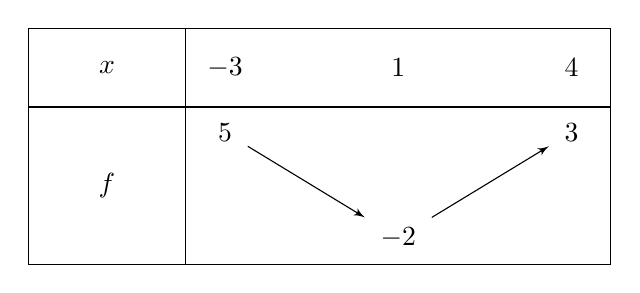
\begin{tikzpicture}
\tkzTabInit[lgt=2,espcl=2.2]{$x$/1,$f$/2}
{$-3$,$1$,$4$}
\tkzTabVar{+/$5$,-/$-2$,+/$3$}
\end{tikzpicture}
\end{center}

\begin{center}
\renewcommand{\arraystretch}{1.5}
\begin{tabular}{|c|ccccc|}
\hline
\(x\) & \(-3\) & & \(1\) & & \(4\) \\
\hline
\(f'(x)\) & & & & & \\
\hline
\end{tabular}
\end{center}

\textbf{Exercice 3 -- \'Etude complète d'une fonction polynomiale \hfill /3}

On considère la fonction \(f\) définie sur \(\mathbb{R}\) par \(f(x)=x^2-4x+1\).

\begin{enumerate}
\item Calculer \(f'(x)\).
\vspace{2cm}
\item En déduire le tableau de signes de \(f'\), puis le tableau de variations de \(f\) sur \(\mathbb{R}\).
\vspace{5.5cm}
\end{enumerate}

\newpage

\interroversion{B}

\textbf{Exercice 1 -- Nombre dérivé lu graphiquement \hfill /1}

La courbe \(\mathcal{C}_f\) d'une fonction \(f\) et sa tangente \(T\) au point \(A\) d'abscisse \(2\) sont tracées ci-dessous.

\`A l'aide du graphique, déterminer \(f'(2)\).

\begin{center}
\tangentegraph{-0.2}{3.3}{\x*\x-3*\x+5}{0}{4.2}{\x+1}
\fill (2,3) circle (2pt);
\node[below right] at (2.05,2.95) {\(A\)};
\node[red] at (0.4,2.8) {\(T\)};
\end{tikzpicture}
\end{center}

Réponse~: \(f'(2)=\) \dotfill

\textbf{Exercice 2 -- Signe de la dérivée et variations \hfill /1}

On donne ci-dessous le tableau de variations d'une fonction \(f\) définie sur \([-2;5]\). En déduire, en le complétant, le tableau de signes de \(f'\) sur ce même intervalle.

\begin{center}
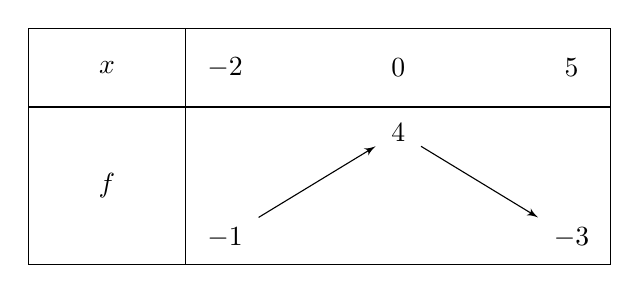
\begin{tikzpicture}
\tkzTabInit[lgt=2,espcl=2.2]{$x$/1,$f$/2}
{$-2$,$0$,$5$}
\tkzTabVar{-/$-1$,+/$4$,-/$-3$}
\end{tikzpicture}
\end{center}

\begin{center}
\renewcommand{\arraystretch}{1.5}
\begin{tabular}{|c|ccccc|}
\hline
\(x\) & \(-2\) & & \(0\) & & \(5\) \\
\hline
\(f'(x)\) & & & & & \\
\hline
\end{tabular}
\end{center}

\textbf{Exercice 3 -- \'Etude complète d'une fonction polynomiale \hfill /3}

On considère la fonction \(f\) définie sur \(\mathbb{R}\) par \(f(x)=-x^2+2x+3\).

\begin{enumerate}
\item Calculer \(f'(x)\).
\vspace{2cm}
\item En déduire le tableau de signes de \(f'\), puis le tableau de variations de \(f\) sur \(\mathbb{R}\).
\vspace{5.5cm}
\end{enumerate}

\newpage

\interroversion{C}

\textbf{Exercice 1 -- Nombre dérivé lu graphiquement \hfill /1}

La courbe \(\mathcal{C}_f\) d'une fonction \(f\) et sa tangente \(T\) au point \(A\) d'abscisse \(1\) sont tracées ci-dessous.

\`A l'aide du graphique, déterminer \(f'(1)\).

\begin{center}
\tangentegraph{0.1}{4}{\x*\x-4*\x+6}{0}{3.7}{5-2*\x}
\fill (1,3) circle (2pt);
\node[above right] at (1.05,3.05) {\(A\)};
\node[red] at (3.3,1.05) {\(T\)};
\end{tikzpicture}
\end{center}

Réponse~: \(f'(1)=\) \dotfill

\textbf{Exercice 2 -- Signe de la dérivée et variations \hfill /1}

On donne ci-dessous le tableau de variations d'une fonction \(f\) définie sur \([-4;3]\). En déduire, en le complétant, le tableau de signes de \(f'\) sur ce même intervalle.

\begin{center}
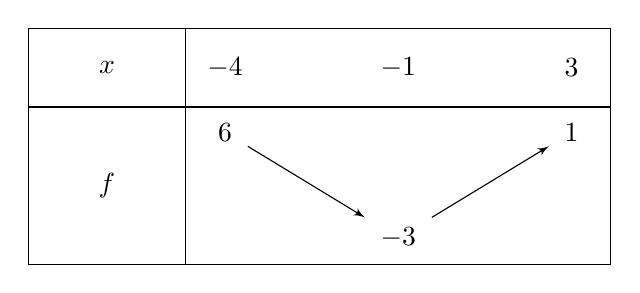
\begin{tikzpicture}
\tkzTabInit[lgt=2,espcl=2.2]{$x$/1,$f$/2}
{$-4$,$-1$,$3$}
\tkzTabVar{+/$6$,-/$-3$,+/$1$}
\end{tikzpicture}
\end{center}

\begin{center}
\renewcommand{\arraystretch}{1.5}
\begin{tabular}{|c|ccccc|}
\hline
\(x\) & \(-4\) & & \(-1\) & & \(3\) \\
\hline
\(f'(x)\) & & & & & \\
\hline
\end{tabular}
\end{center}

\textbf{Exercice 3 -- \'Etude complète d'une fonction polynomiale \hfill /3}

On considère la fonction \(f\) définie sur \(\mathbb{R}\) par \(f(x)=2x^2-4x-1\).

\begin{enumerate}
\item Calculer \(f'(x)\).
\vspace{2cm}
\item En déduire le tableau de signes de \(f'\), puis le tableau de variations de \(f\) sur \(\mathbb{R}\).
\vspace{5.5cm}
\end{enumerate}

\newpage

\interroversion{D}

\textbf{Exercice 1 -- Nombre dérivé lu graphiquement \hfill /1}

La courbe \(\mathcal{C}_f\) d'une fonction \(f\) et sa tangente \(T\) au point \(A\) d'abscisse \(3\) sont tracées ci-dessous.

\`A l'aide du graphique, déterminer \(f'(3)\).

\begin{center}
\tangentegraph{0.5}{4.5}{\x*\x-5*\x+7}{1}{5}{\x-2}
\fill (3,1) circle (2pt);
\node[below right] at (3.05,0.95) {\(A\)};
\node[red] at (1,1) {\(T\)};
\end{tikzpicture}
\end{center}

Réponse~: \(f'(3)=\) \dotfill

\textbf{Exercice 2 -- Signe de la dérivée et variations \hfill /1}

On donne ci-dessous le tableau de variations d'une fonction \(f\) définie sur \([-3;2]\). En déduire, en le complétant, le tableau de signes de \(f'\) sur ce même intervalle.

\begin{center}
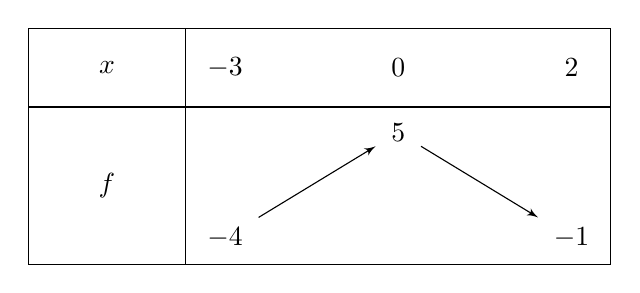
\begin{tikzpicture}
\tkzTabInit[lgt=2,espcl=2.2]{$x$/1,$f$/2}
{$-3$,$0$,$2$}
\tkzTabVar{-/$-4$,+/$5$,-/$-1$}
\end{tikzpicture}
\end{center}

\begin{center}
\renewcommand{\arraystretch}{1.5}
\begin{tabular}{|c|ccccc|}
\hline
\(x\) & \(-3\) & & \(0\) & & \(2\) \\
\hline
\(f'(x)\) & & & & & \\
\hline
\end{tabular}
\end{center}

\textbf{Exercice 3 -- \'Etude complète d'une fonction polynomiale \hfill /3}

On considère la fonction \(f\) définie sur \(\mathbb{R}\) par \(f(x)=-x^2-2x+4\).

\begin{enumerate}
\item Calculer \(f'(x)\).
\vspace{2cm}
\item En déduire le tableau de signes de \(f'\), puis le tableau de variations de \(f\) sur \(\mathbb{R}\).
\vspace{5.5cm}
\end{enumerate}

\end{document}
